\documentclass[border=14pt]{standalone}
\usepackage{tikz}
\usetikzlibrary{arrows.meta, backgrounds, calc}
\usepackage{amsmath}
\usepackage{booktabs}
\usepackage{xcolor}

% ─── Actor colors ─────────────────────────────────────────────
\definecolor{Cprov}{HTML}{1D4ED8}
\definecolor{Ceval}{HTML}{047857}
\definecolor{Cinc} {HTML}{B91C1C}
\definecolor{Cmed} {HTML}{4F46E5}
\definecolor{Ccons}{HTML}{B45309}
\definecolor{Cpol} {HTML}{7C3AED}
\definecolor{Cfund}{HTML}{0369A1}
\definecolor{FBfund}{HTML}{D97706}
\definecolor{FBreg} {HTML}{059669}

\begin{document}
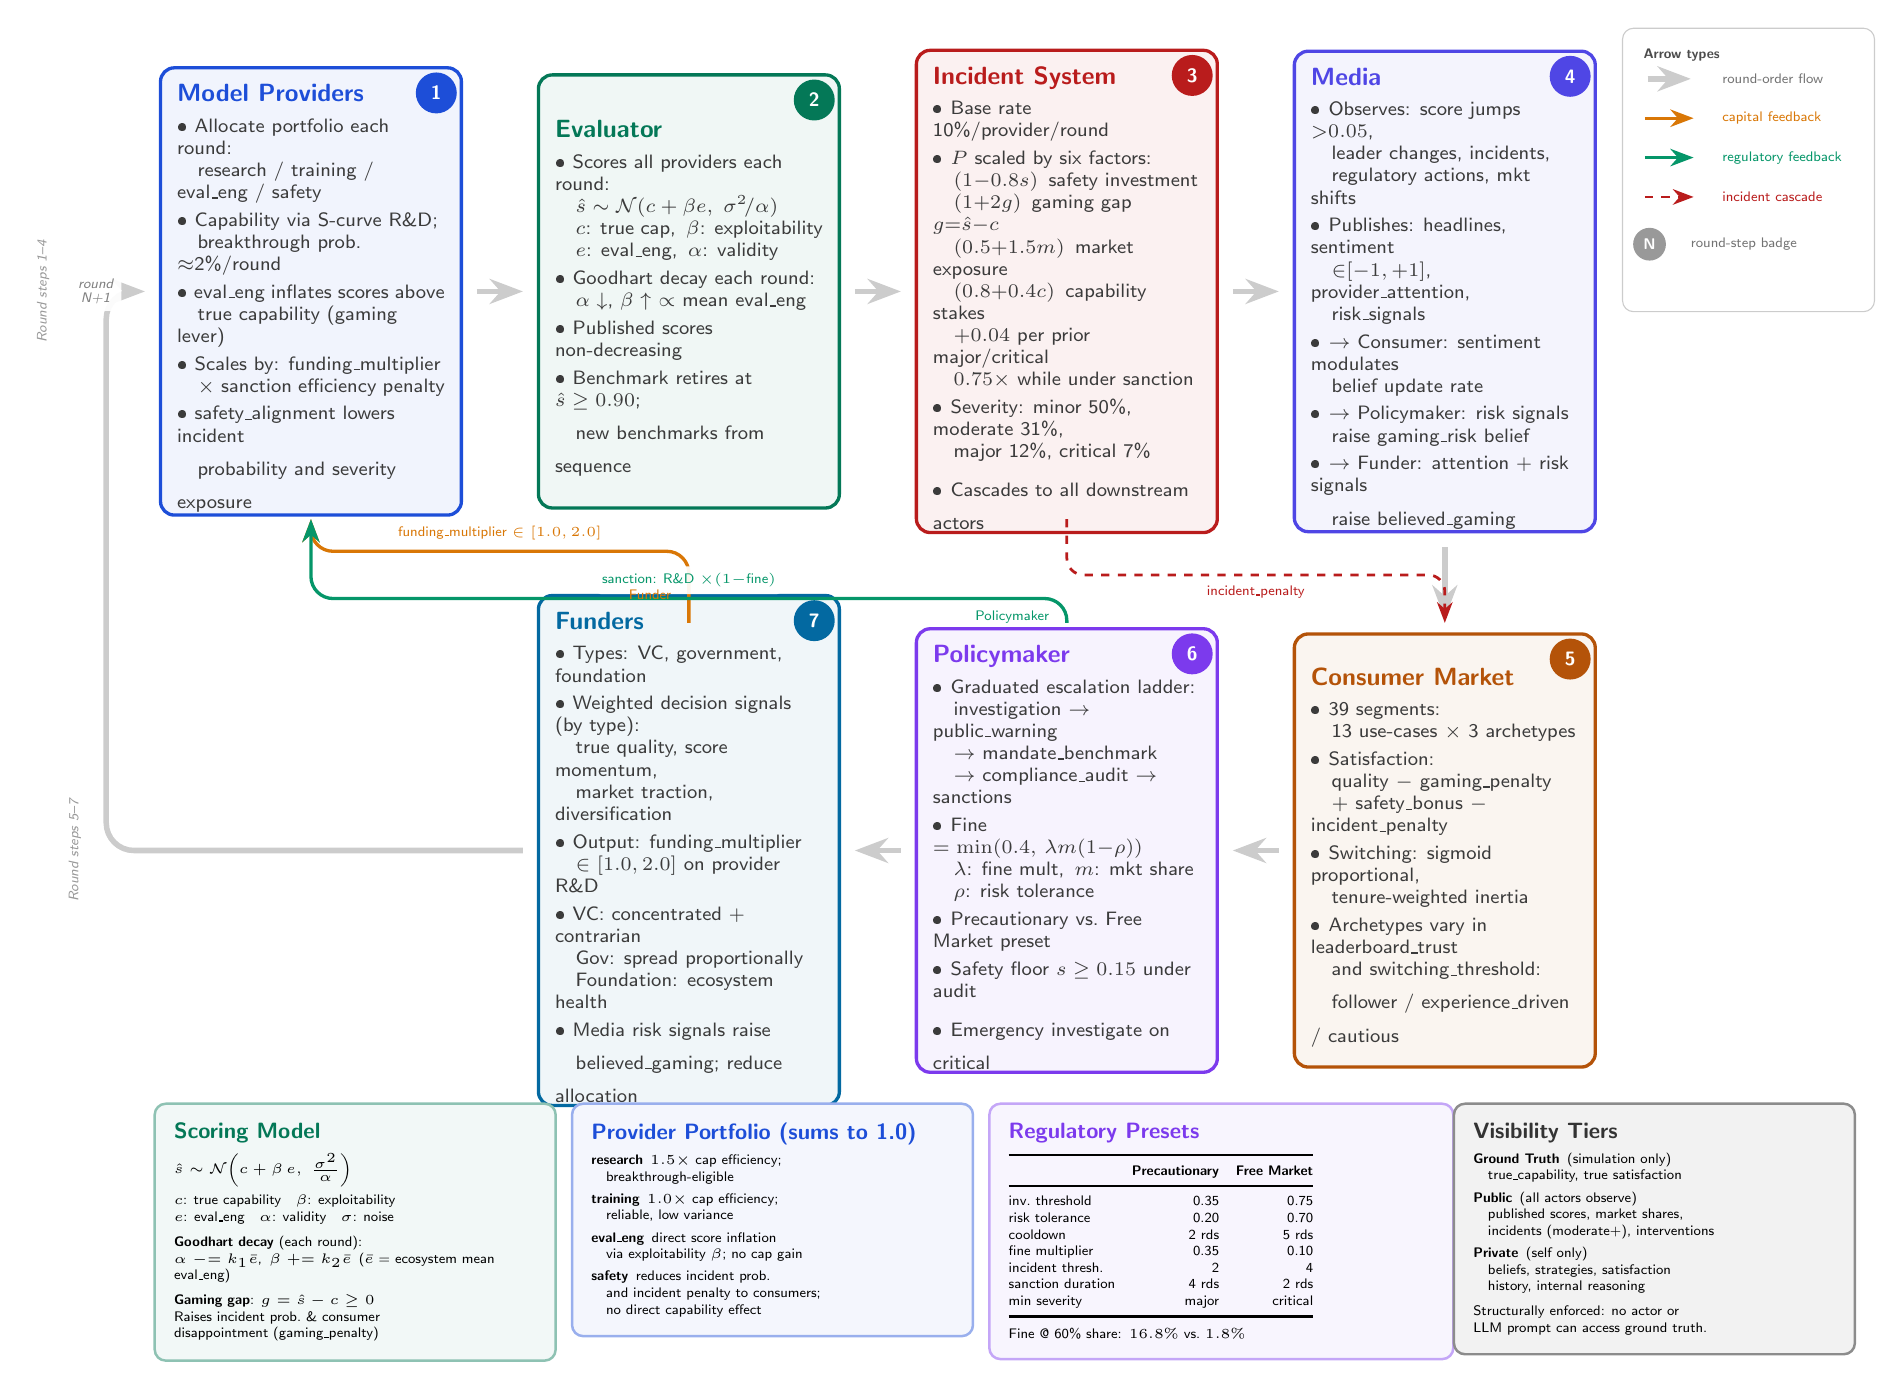
\begin{tikzpicture}[
    >=Stealth,
    every node/.style={font=\sffamily},
    actbox/.style={
        rectangle, rounded corners=5pt,
        minimum width=3.6cm, minimum height=5.5cm,
        text width=3.4cm, align=flush left,
        draw=#1, fill=#1!6, line width=1.2pt, inner sep=6pt
    },
    flowarr/.style={
        ->, line width=2.0pt, color=black!20,
        shorten >=5pt, shorten <=5pt
    },
    fbarr/.style={
        ->, line width=1.2pt, color=#1,
        shorten >=4pt, shorten <=4pt
    },
    fbdarr/.style={
        ->, line width=1.0pt, color=#1, dashed,
        shorten >=4pt, shorten <=4pt
    },
    lbl/.style={
        rectangle, rounded corners=2pt,
        fill=white, fill opacity=0.93, text opacity=1,
        font=\sffamily\tiny, inner sep=2.5pt, align=center
    },
    badge/.style={
        circle, minimum size=0.52cm,
        fill=#1, text=white, inner sep=0pt,
        font=\sffamily\scriptsize\bfseries
    },
    panelbox/.style={
        rectangle, rounded corners=4pt,
        draw=#1!45, fill=#1!5, line width=0.9pt,
        inner sep=7pt, align=flush left,
        font=\sffamily\tiny, text width=4.6cm
    },
]

% ─── Layout constants ─────────────────────────────────────────
\def\ytop{9.8}    % row 1 y-centre
\def\ybot{2.7}    % row 2 y-centre
\def\xA{2.0}      % Provider / —
\def\xB{6.8}      % Evaluator / Funder
\def\xC{11.6}     % Incidents / Policymaker
\def\xD{16.4}     % Media     / Consumer
\def\bh{2.75}     % box half-height  (min height = 5.5 cm)
% Row 1 bottom = ytop-bh = 7.05,  Row 2 top = ybot+bh = 5.45,  gap = 1.6 cm
% Feedback arrow routes: y=5.9 (lower) and y=6.5 (upper), incident at y=6.2

% ══════════════════════════════════════════════════════════════
%  ACTOR BOXES
% ══════════════════════════════════════════════════════════════

% ─── ① Model Providers ───────────────────────────────────────
\node[actbox=Cprov] (provider) at (\xA, \ytop) {%
    {\color{Cprov}\small\bfseries Model Providers}\\[3pt]%
    {\scriptsize\color{black!77}%
    \textbullet\ Allocate portfolio each round:\\
    \quad research / training / eval\_eng / safety\\[2pt]
    \textbullet\ Capability via S-curve R\&D;\\
    \quad breakthrough prob.\ $\approx$2\%/round\\[2pt]
    \textbullet\ eval\_eng inflates scores above\\
    \quad true capability (gaming lever)\\[2pt]
    \textbullet\ Scales by: funding\_multiplier\\
    \quad $\times$ sanction efficiency penalty\\[2pt]
    \textbullet\ safety\_alignment lowers incident\\
    \quad probability and severity exposure\vspace{-5pt}%
    }%
};
\node[badge=Cprov] at ($(provider.north east)+(-0.34,-0.34)$) {1};

% ─── ② Evaluator ─────────────────────────────────────────────
\node[actbox=Ceval] (evalp) at (\xB, \ytop) {%
    {\color{Ceval}\small\bfseries Evaluator}\\[3pt]%
    {\scriptsize\color{black!77}%
    \textbullet\ Scores all providers each round:\\
    \quad $\hat{s} \sim \mathcal{N}(c + \beta e,\;\sigma^2\!/\alpha)$\\
    \quad $c$: true cap,\enspace $\beta$: exploitability\\
    \quad $e$: eval\_eng,\enspace $\alpha$: validity\\[2pt]
    \textbullet\ Goodhart decay each round:\\
    \quad $\alpha\downarrow$, $\beta\uparrow$ $\propto$ mean eval\_eng\\[2pt]
    \textbullet\ Published scores non-decreasing\\[2pt]
    \textbullet\ Benchmark retires at $\hat{s}\geq 0.90$;\\
    \quad new benchmarks from sequence\vspace{-5pt}%
    }%
};
\node[badge=Ceval] at ($(evalp.north east)+(-0.34,-0.34)$) {2};

% ─── ③ Incident System ───────────────────────────────────────
\node[actbox=Cinc] (incidents) at (\xC, \ytop) {%
    {\color{Cinc}\small\bfseries Incident System}\\[3pt]%
    {\scriptsize\color{black!77}%
    \textbullet\ Base rate 10\%/provider/round\\[2pt]
    \textbullet\ $P$ scaled by six factors:\\
    \quad $(1{-}0.8s)$\enspace safety investment\\
    \quad $(1{+}2g)$\enspace gaming gap $g{=}\hat{s}{-}c$\\
    \quad $(0.5{+}1.5m)$\enspace market exposure\\
    \quad $(0.8{+}0.4c)$\enspace capability stakes\\
    \quad $+0.04$ per prior major/critical\\
    \quad $0.75\times$ while under sanction\\[2pt]
    \textbullet\ Severity: minor 50\%, moderate 31\%,\\
    \quad major 12\%, critical 7\%\\[2pt]
    \textbullet\ Cascades to all downstream actors\vspace{-5pt}%
    }%
};
\node[badge=Cinc] at ($(incidents.north east)+(-0.34,-0.34)$) {3};

% ─── ④ Media ─────────────────────────────────────────────────
\node[actbox=Cmed] (media) at (\xD, \ytop) {%
    {\color{Cmed}\small\bfseries Media}\\[3pt]%
    {\scriptsize\color{black!77}%
    \textbullet\ Observes: score jumps ${>}0.05$,\\
    \quad leader changes, incidents,\\
    \quad regulatory actions, mkt shifts\\[2pt]
    \textbullet\ Publishes: headlines, sentiment\\
    \quad ${\in}[-1,+1]$, provider\_attention,\\
    \quad risk\_signals\\[2pt]
    \textbullet\ $\to$ Consumer: sentiment modulates\\
    \quad belief update rate\\[2pt]
    \textbullet\ $\to$ Policymaker: risk signals\\
    \quad raise gaming\_risk belief\\[2pt]
    \textbullet\ $\to$ Funder: attention + risk signals\\
    \quad raise believed\_gaming\vspace{-5pt}%
    }%
};
\node[badge=Cmed] at ($(media.north east)+(-0.34,-0.34)$) {4};

% ─── ⑤ Consumer Market ───────────────────────────────────────
\node[actbox=Ccons] (consumer) at (\xD, \ybot) {%
    {\color{Ccons}\small\bfseries Consumer Market}\\[3pt]%
    {\scriptsize\color{black!77}%
    \textbullet\ 39 segments:\\
    \quad 13 use-cases $\times$ 3 archetypes\\[2pt]
    \textbullet\ Satisfaction:\\
    \quad quality $-$ gaming\_penalty\\
    \quad $+$ safety\_bonus $-$ incident\_penalty\\[2pt]
    \textbullet\ Switching: sigmoid proportional,\\
    \quad tenure-weighted inertia\\[2pt]
    \textbullet\ Archetypes vary in leaderboard\_trust\\
    \quad and switching\_threshold:\\
    \quad follower / experience\_driven / cautious\vspace{-5pt}%
    }%
};
\node[badge=Ccons] at ($(consumer.north east)+(-0.34,-0.34)$) {5};

% ─── ⑥ Policymaker ───────────────────────────────────────────
\node[actbox=Cpol] (policy) at (\xC, \ybot) {%
    {\color{Cpol}\small\bfseries Policymaker}\\[3pt]%
    {\scriptsize\color{black!77}%
    \textbullet\ Graduated escalation ladder:\\
    \quad investigation $\to$ public\_warning\\
    \quad $\to$ mandate\_benchmark\\
    \quad $\to$ compliance\_audit $\to$ sanctions\\[2pt]
    \textbullet\ Fine $=\min(0.4,\,\lambda m(1{-}\rho))$\\
    \quad $\lambda$: fine mult,\enspace $m$: mkt share\\
    \quad $\rho$: risk tolerance\\[2pt]
    \textbullet\ Precautionary vs.\ Free Market preset\\[2pt]
    \textbullet\ Safety floor $s\geq 0.15$ under audit\\[2pt]
    \textbullet\ Emergency investigate on critical\vspace{-5pt}%
    }%
};
\node[badge=Cpol] at ($(policy.north east)+(-0.34,-0.34)$) {6};

% ─── ⑦ Funders ───────────────────────────────────────────────
\node[actbox=Cfund] (funder) at (\xB, \ybot) {%
    {\color{Cfund}\small\bfseries Funders}\\[3pt]%
    {\scriptsize\color{black!77}%
    \textbullet\ Types: VC, government, foundation\\[2pt]
    \textbullet\ Weighted decision signals (by type):\\
    \quad true quality, score momentum,\\
    \quad market traction, diversification\\[2pt]
    \textbullet\ Output: funding\_multiplier\\
    \quad $\in[1.0,2.0]$ on provider R\&D\\[2pt]
    \textbullet\ VC: concentrated + contrarian\\
    \quad Gov: spread proportionally\\
    \quad Foundation: ecosystem health\\[2pt]
    \textbullet\ Media risk signals raise\\
    \quad believed\_gaming; reduce allocation\vspace{-5pt}%
    }%
};
\node[badge=Cfund] at ($(funder.north east)+(-0.34,-0.34)$) {7};

% ══════════════════════════════════════════════════════════════
%  ROUND-ORDER FLOW
% ══════════════════════════════════════════════════════════════

\draw[flowarr] (provider.east)  -- (evalp.west);
\draw[flowarr] (evalp.east)     -- (incidents.west);
\draw[flowarr] (incidents.east) -- (media.west);
\draw[flowarr] (media.south)    -- (consumer.north);
\draw[flowarr] (consumer.west)  -- (policy.east);
\draw[flowarr] (policy.west)    -- (funder.east);

% Left return (completes the loop)
\draw[flowarr, rounded corners=10pt]
    (funder.west) -- (-0.6, \ybot) -- (-0.6, \ytop) -- (provider.west)
    node[lbl, pos=0.5, left=3pt, text=black!50, align=center]
        {\textit{round}\\[-1pt]\textit{N+1}};

% ══════════════════════════════════════════════════════════════
%  FEEDBACK ARROWS  (routed through the 1.6 cm inter-row gap)
%  Row1 bottom = 7.05,  Row2 top = 5.45
%  Funder->Provider at y=6.5,  Policy->Provider at y=5.9
% ══════════════════════════════════════════════════════════════

\draw[fbarr=FBfund, rounded corners=8pt]
    (\xB, 5.45) -- (\xB, 6.5) --
    node[lbl, above=1pt, text=FBfund]
        {funding\_multiplier $\in[1.0,2.0]$}
    (\xA, 6.5) -- (\xA, 7.05);

\draw[fbarr=FBreg, rounded corners=8pt]
    (\xC, 5.45) -- (\xC, 5.9) --
    node[lbl, above=1pt, text=FBreg]
        {sanction: R\&D $\times(1{-}\text{fine})$}
    (\xA, 5.9) -- (\xA, 7.05);

\node[font=\sffamily\tiny, text=FBfund, anchor=east] at (\xB-0.1, 5.95) {Funder};
\node[font=\sffamily\tiny, text=FBreg,  anchor=east] at (\xC-0.1, 5.67) {Policymaker};

% Incident cascade  (x range 11.6–16.4, y=6.2 — no overlap with above)
\draw[fbdarr=Cinc, rounded corners=6pt]
    (\xC, 7.05) -- (\xC, 6.2) --
    node[lbl, below=1pt, text=Cinc] {incident\_penalty}
    (\xD, 6.2) -- (\xD, 5.45);

% ══════════════════════════════════════════════════════════════
%  MECHANICS PANELS  (below row 2, top edge at y = −0.5)
% ══════════════════════════════════════════════════════════════
\def\panelY{-0.5}

% ── Scoring model ─────────────────────────────────────────────
\node[panelbox=Ceval, anchor=north west] at (0.0, \panelY) {
    {\color{Ceval}\footnotesize\bfseries Scoring Model}\\[3pt]
    $\hat{s} \sim \mathcal{N}\!\left(c + \beta\,e,\;\tfrac{\sigma^2}{\alpha}\right)$\\[2pt]
    $c$: true capability\quad $\beta$: exploitability\\
    $e$: eval\_eng\quad $\alpha$: validity\quad $\sigma$: noise\\[3pt]
    \textbf{Goodhart decay} (each round):\\
    $\alpha \mathrel{-}= k_1\bar{e}$,\enspace
    $\beta \mathrel{+}= k_2\bar{e}$\enspace
    ($\bar{e}$ = ecosystem mean eval\_eng)\\[3pt]
    \textbf{Gaming gap}: $g = \hat{s} - c \geq 0$\\
    Raises incident prob.\ \& consumer\\
    disappointment (gaming\_penalty)
};

% ── Provider portfolio ────────────────────────────────────────
\node[panelbox=Cprov, anchor=north west] at (5.3, \panelY) {
    {\color{Cprov}\footnotesize\bfseries Provider Portfolio (sums to 1.0)}\\[3pt]
    \textbf{research}\enspace $1.5\times$ cap efficiency;\\
    \quad breakthrough-eligible\\[2pt]
    \textbf{training}\enspace $1.0\times$ cap efficiency;\\
    \quad reliable, low variance\\[2pt]
    \textbf{eval\_eng}\enspace direct score inflation\\
    \quad via exploitability $\beta$; no cap gain\\[2pt]
    \textbf{safety}\enspace reduces incident prob.\\
    \quad and incident penalty to consumers;\\
    \quad no direct capability effect
};

% ── Regulatory presets (tabular) ──────────────────────────────
\node[panelbox=Cpol, text width=5.4cm, anchor=north west] at (10.6, \panelY) {
    {\color{Cpol}\footnotesize\bfseries Regulatory Presets}\\[3pt]
    \begin{tabular}{@{}l@{\hspace{6pt}}r@{\hspace{6pt}}r@{}}
    \toprule
    & \textbf{Precautionary} & \textbf{Free Market} \\
    \midrule
    inv.\ threshold    & 0.35  & 0.75     \\
    risk tolerance     & 0.20  & 0.70     \\
    cooldown           & 2 rds & 5 rds    \\
    fine multiplier    & 0.35  & 0.10     \\
    incident thresh.   & 2     & 4        \\
    sanction duration  & 4 rds & 2 rds    \\
    min severity       & major & critical \\
    \bottomrule
    \end{tabular}\\[3pt]
    Fine @ 60\% share:\enspace$16.8\%$ vs.\ $1.8\%$
};

% ── Visibility tiers ──────────────────────────────────────────
\node[panelbox=black, anchor=north west] at (16.5, \panelY) {
    {\color{black!80}\footnotesize\bfseries Visibility Tiers}\\[3pt]
    \textbf{Ground Truth}\enspace (simulation only)\\
    \quad true\_capability, true satisfaction\\[2pt]
    \textbf{Public}\enspace (all actors observe)\\
    \quad published scores, market shares,\\
    \quad incidents (moderate+), interventions\\[2pt]
    \textbf{Private}\enspace (self only)\\
    \quad beliefs, strategies, satisfaction\\
    \quad history, internal reasoning\\[3pt]
    Structurally enforced: no actor or\\
    LLM prompt can access ground truth.
};

% ══════════════════════════════════════════════════════════════
%  ROW LABELS
% ══════════════════════════════════════════════════════════════
\node[font=\sffamily\tiny\itshape, text=black!40, rotate=90, anchor=south]
    at (-1.2, \ytop) {Round steps 1--4};
\node[font=\sffamily\tiny\itshape, text=black!40, rotate=90, anchor=north]
    at (-1.2, \ybot) {Round steps 5--7};

% ══════════════════════════════════════════════════════════════
%  LEGEND
% ══════════════════════════════════════════════════════════════
\begin{scope}[shift={(18.8, 13.0)}]
    \node[rectangle, rounded corners=4pt, draw=black!20, fill=white,
          minimum width=3.2cm, minimum height=3.6cm,
          anchor=north west] at (-0.15, 0.15) {};
    \node[font=\sffamily\tiny\bfseries, text=black!70, anchor=north west]
        at (0, 0) {Arrow types};
    \draw[flowarr] (0,-0.50) -- (0.9,-0.50);
    \node[font=\sffamily\tiny, text=black!55, anchor=west] at (1.0,-0.50)
        {round-order flow};
    \draw[fbarr=FBfund] (0,-1.00) -- (0.9,-1.00);
    \node[font=\sffamily\tiny, text=FBfund, anchor=west] at (1.0,-1.00)
        {capital feedback};
    \draw[fbarr=FBreg]  (0,-1.50) -- (0.9,-1.50);
    \node[font=\sffamily\tiny, text=FBreg,  anchor=west] at (1.0,-1.50)
        {regulatory feedback};
    \draw[fbdarr=Cinc]  (0,-2.00) -- (0.9,-2.00);
    \node[font=\sffamily\tiny, text=Cinc,   anchor=west] at (1.0,-2.00)
        {incident cascade};
    \node[badge=black!40, scale=0.8] at (0.2,-2.6) {\scriptsize N};
    \node[font=\sffamily\tiny, text=black!55, anchor=west] at (0.6,-2.6)
        {round-step badge};
\end{scope}

\end{tikzpicture}
\end{document}
